\chapter{Load Generating Tool}
	\label{scale-load-generator}
As mentioned in chapter \ref{technological background}, existing load generating tools requires comparatively powerful computing unit to host them. In this project, it is not realistic to host such a vigorous load generator because of the cost and complexity from extra virtual machine to be installed. Additionally, if client and server are running in the same cluster, unwelcome network overhead can be avoided in some extent. Although self implemented load generator is limited in its capacity, it can be made up through scaling the load generator instance. As figure  \ref{scale-load-generator} shows, enough load can be brought about by parallel running multiple instances.
\begin{figure}[h]
	\centering
	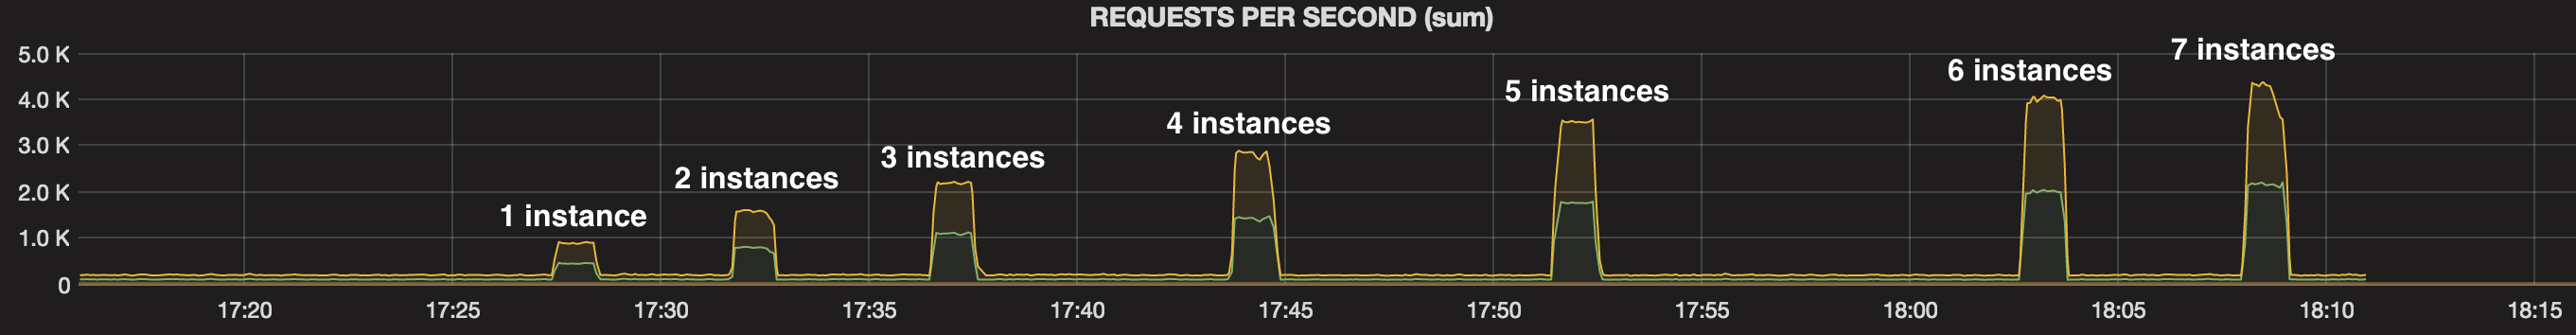
\includegraphics[width=12cm]{scale-load-generator}
	\caption{Load produced from different number of instances}
	\label{scale-load-generator}
\end{figure}

\section{Load generator - a self implemented scalable client}
A simple load generator is implemented in this project as a node application. It sends requests with unique correlation id to the server, records the response time and stores them in database at the end of load generating. Application is deployed to cloud foundry and uses PostgreSQL backing service. A time-out mechanism is added to make sure load is generated in the given time frame. Except for producing fancy graphic analysis results, it pretty much accomplishes every thing a load generating tool can do. It is more flexible to work with raw data anyway.
\missingfigure{Add figure for node application for load generator}

\subsection{Features}
\label{load generator}
The majority of the load testing frameworks choose to generate a fixed number of total requests with given amount of concurrencies.  For example, a typical \textit{JMeter} test plan configures parameter \textit{Number of Threads} as concurrent virtual users. Through\textit{Loop Count}, the same concurrency is repeated so to reach the total number of requests. \textit{Hey} defines the total requests and concurrency degree then carry out the load generating accordingly. The same principle behind them is that the period of time during which the tests are carried out is not measured only the response time of individual request. So many requests shall be sent either ended with successful transaction or landed in error because of timeout or other various reasons. \\
The load generator used in this project produces load in two ways. One implementation also generates the load with a fixed number of requests. Another implementation brings about parallel requests in a fixed time frame, for example in one minute. The application will first pile up requests to a predefined parallel parameter. Whenever a request is successfully returned, a new one will be created to maintain the total parallel requests. Since the load testing is executed in an cloud environment where there are productive applications, define a relatively short time frame reduces influence on others.\\
The proxy server limitation is discussed in \ref{haproxy}. At the beginning the requests on the server was always brought about through establishing new connections. This has quickly hit the limit of what the HAProxy can handle. To workaround it, the started connections are kept alive and reused. Although HAProxy has a strange setting of cutting off the connection after a period of time, when the time expanse of test is not set to this limit, all things work perfectly. 

\subsection{Limitations}
Since load generator is deployed as a worker in Cloud Foundry, it has little choice over database selection. In this project, a docker container version of database is used owing to the fact that other dedicated backing services are not free of charge. There are times container is simply overloaded and refuse to store any more data. \\
Secondly, load generator can be resource consuming as already discussed. In Cloud Foundry, some organization or space has only so much memory to provide. It could be hard to scale the load generator to ideal capacity.In this thesis, for a period of time the load testing is conducted in a staging landscape of Cloud Foundry with a limited space quota of 10 G memory. Imagine all the applications and load generators scaling together, the space limit is easily exceeded. \\
Last but not the least, there is a chance the load generator is running on the same node as applications which will directly influence the CPU share the application could obtain and result in tainted test results. 

